% Created 2017-03-12 Sun 15:58
\documentclass[12pt]{amsart}
                        \usepackage[all]{pabmacros}
\usepackage[utf8]{inputenc}
\usepackage[T1]{fontenc}
\usepackage{fixltx2e}
\usepackage{graphicx}
\usepackage{longtable}
\usepackage{float}
\usepackage{wrapfig}
\usepackage[normalem]{ulem}
\usepackage{textcomp}
\usepackage{marvosym}
\usepackage[nointegrals]{wasysym}
\usepackage{latexsym}
\usepackage{amssymb}
\usepackage{amstext}
\usepackage{hyperref}
\tolerance=1000
\usepackage{amsmath}
\usepackage[bibstyle=alphabetic,citestyle=alphabetic,backend=bibtex]{biblatex}
\makeatletter
\def\blx@maxline{77}
\makeatother
\bibliography{refs}
\AtEveryBibitem{\clearfield{doi}}
\AtEveryBibitem{\clearfield{url}}
\AtEveryBibitem{\clearfield{issn}}
\renewcommand*{\bibfont}{\footnotesize}
\renewcommand\maketitle{}
\usepackage{enumitem}
\usepackage{setspace}
\usepackage[margin = 6mm]{geometry}
\pagenumbering{gobble}
\pagestyle{empty}
\renewcommand*{\bibfont}{\footnotesize}
\date{}
\title{D1 Project Description}
\hypersetup{
  pdfkeywords={},
  pdfsubject={},
  pdfcreator={Emacs 24.5.1 (Org mode 8.2.10)}}
\begin{document}

\maketitle


\smallskip\noindent{\Large\textbf{\textsc{Project Title}}}
\label{sec-1}
Analysis and geometric techniques for fully non-linear problems in geometry and PDE.

\smallskip\noindent{\Large\textbf{\textsc{Aims And Background}}}
\label{sec-2}
Geometric evolution equations are ubiquitous and have been used to extraordinary effect in solving many important problems in geometry and topology.  Perhaps the most famous, is the resolution of the \poincare{} conjecture by Hamilton and Perelman \cite{MR2334563}.  Other, equally striking (mathematically, perhaps if not sensationally) results are the $1/4$ pinched sphere theorems (see \cite{MR2738904} for a recent survey article or \cite{MR2760593} for a more comprehensive account), Cao's proof of the Calabi conjecture \cite{MR799272} and two different proofs of the Riemannian Penrose inequality \cite{MR1916951, MR1908823}.

Such results depend crucially on careful analysis of asymptotics and singularity formation. Innovative isoperimetric comparison techniques were introduced in \cite{MR2729306,MR2794630,MR2843240,pbthesis,Bryan} Prof. Ben Andrews and Dr. Bryan to obtaining very direct proofs that arbitrary initial configurations converge smoothly to the model, constant curvature configuration. These results then yield proofs of the famous uniformisation theorem classifying all closed surfaces by genus, and also the classical isoperimetric inequality stating that among all planar figures of a given area, the circle has the least perimeter.

In three dimensions, the \poincare{} conjecture mentioned above fits into a larger scheme known as the Thurston Geometrisation Conjecture \cite{MR2334563} and this is in fact what Hamilton and Perelman proved. Roughly speaking, this conjecture says any compact three dimensional manifold may be decomposed into smaller simpler pieces, and that each of these pieces is one of eight possible types - the so called \emph{Prime manifolds}. The manifolds include in particular the standard Euclidean, Spherical and Hyperbolic geometries. Such a decomposition allows one to study these pieces separately and is a great boon given the otherwise complex topology of three-manifolds.

In particular, the negatively curved manifolds form the largest class of prime manifolds and deeper questions on these objects are not well suited to Hamilton's and Perelman's approach based on the Ricci flow which is most effective in positive curvature. To remedy the situation Hamilton and Chow introduced the Cross Curvature Flow \cite{MR2055396}, a fully non-linear equation that preserves the property of negative curvature. Only scattered results are known for this flow so far, but all support the conjecture that any negatively curved manifold will smoothly converge to a constant curvature, \emph{hyperbolic manifold}. Such a result would imply that any negatively curved manifold may be seen as a perturbation of the constant curvature hyperbolic manifold thus revealing hidden simplicity in the topology of these mysterious negatively curved spaces.

Another approach to these types of problems is to study ancient solutions, solitons and the closely related Harnack inequality. Such an approach is recognised as extremely important as evidenced by the awarding of DFG-Grant SCHE 1879/1-1 "Harnack inequalities for curvature flows and applications" to Dr. Bryan's collaborator Dr. Julian Scheuer. It has been known for some time that ancient solutions, and solitons in particular model singularity formation and hence studying such special solutions lends tremendous insight into the sort of problems described above. Dr. Mohammad Ivaki, Dr. Julian Scheuer and Dr. Bryan have developed considerable apparatus \cite{BIS4,2016arXiv160401694B,2015arXiv150802821B,2015arXiv151203374B} for studying ancient solutions and obtaining Harnack inequalities in Riemannian backgrounds, a very surprising and difficult result given the non-linearity introduced by the curvature of the background space. Moreover, very strong classification results for ancient solutions were obtained via geometric methods showing for example that \emph{for any heat-type geometric flow on the sphere}, the only ancient, convex solutions are spherical caps, suggesting that in positive curvature, the space of such solutions is very rigid.

The \textbf{aim} of this proposal is to extend the innovative and powerful methods described above to a broad variety of actively studied problems with applications to hyperbolic manifold topology, isoperimetric inequalities, and minimal surfaces.

\begin{enumerate}[label=\textbf{(\Alph*)}]
\item Examine the connections between geometric evolution equations and isoperimetric comparisons, obtaining comparisons and quantifying asymptotic singularity formation for a variety of geometric evolution equations (joint with Prof. Ben Andrews and Prof Mariel \saez{}).
\item Develop a theory of the Cross Curvature Flow and apply it to obtain a topological classification of hyperbolic manifolds (joint with Dr. Mohammad Ivaki and Dr. Julian Scheuer).
\item Perform stability analysis of ancient solutions to curvature flows and classify such solutions. In particular, apply these results to obtain conjectured area estimates for minimal surfaces and explore the connections between curvature flows and the conformal geometry of the sphere (joint with Dr. Mohammad Ivaki and Dr. Julian Scheuer).
\end{enumerate}

\noindent More detailed aims and background for each project follow.

\noindent\textbf{Project A: Isoperimetric Comparisons}
\label{sec-2-1}
The classic isoperimetric inequality states that the figure in the plane with least perimeter bounding a given area is a circle. This result has been known since antiquity by the name Dido's problem who was tasked with enclosing the greatest amount of area given a fixed perimeter. In the 20th century, isoperimetric inequalities comparing the perimeter of a figure with it's enclosed area were obtained for constant curvature spaces. The situation is illustrated in figure \ref{fg:const_curve_isoperimetric}. The latter part of the 20th century and early parts of this century saw the beginning of results for spaces with variable curvature \cite{MR1699261,MR1661278,MR1883725}.

\begin{figure}[htb]
\centering
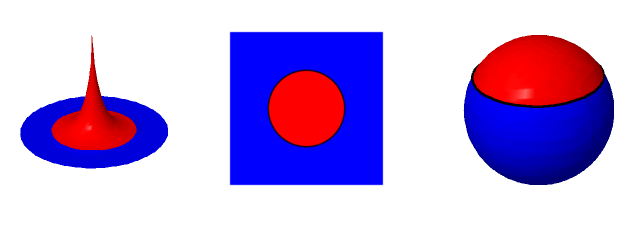
\includegraphics[width=0.7\textwidth]{img/const_curve.png}
\caption{\label{fg:const_curve_isoperimetric}From left to right: an isoperimetric region (red) in a constant negative curvature surface, the plane, and the sphere.}
\end{figure}

The isoperimetric profile of a Riemannian manifold was introduced in the 1980's \cite{MR875084,MR999971} to study isoperimetric inequalities on Riemannian manifolds. It is a function that gives the least perimeter bounding a given area $x$, and is defined by
\[
I(x) = \inf\{\operatorname{Area} (\bdry{\Omega}) : \operatorname{Vol}(\Omega) = x\}.
\]
Thee sharpest possible isoperimetric inequality on a Riemannian manifold comparing the $n-1$ dimensional area of a figure with it's enclosed $n$ dimensional volume is recorded in $I$:
\[
\operatorname{Area}_{n-1} (\bdry{\Omega}) \geq I(\operatorname{Vol}_n(\Omega))
\]
For example the classic isoperimetric inequality implies that the isoperimetric profile of the plane is $I_{\RR^2}(x) = \sqrt{4\pi x}$, of the $2$-sphere is $I_{\sphere^2}(x) = \sqrt{4\pi x - x^2}$ and of the hyperbolic plane is $I_{\HH^2} (x) = \sqrt{4\pi x + x^2}$. We have the obvious inequalities,
\[
I_{\sphere^2} < I_{\RR^2} < I_{\HH^2}.
\]
In general, for a simply connected (no holes) constant curvature surface with curvature $K_0$ we have,
\[
I_{K_0}(x) = \sqrt{4\pi x - K_0 x^2},
\]
exhibiting the general expected phenomena that increasing curvature allows one to enclose more area for a given perimeter which is also evident in figure \ref{fg:const_curve_isoperimetric}. A variant of Dido's problem says that she encircled a hill (positive curvature) to obtain more area compared with a flat plane (zero curvature) suggesting that she was qualitatively aware of the connection to curvature.

The connection between curvature and isoperimetric comparisons was exploited by Prof. Ben Andrews and Dr. Bryan in \cite{MR2729306,MR2843240,pbthesis,Bryan} as mentioned above to obtain curvature bounds and prove convergence results for the Ricci flow on closed surfaces and the Curve Shortening Flow.

A major outstanding conjecture in this area is the Aubin-Cartan-Hadamard conjecture \cite{MR936419} stating that for simply connected, non-positively curved manifolds, the expected comparison where increasing curvature decreases $I$ holds: if the sectional curvature is bounded above by $K_0 \leq 0$, then $I(x) \geq I_{K_0}$. Classically, this has been proven generally in dimensions two and three and in dimension four when $K_0 = 0$ (see \cite{MR2167269}), but still remains outstanding in general.

For a curve in the plane, similar to the isoperimetric profile, we may define the \emph{chord-arc profile} as the least distance between any points on the curve of a given arc-length along the curve:
\[
Z(x) = \inf\{d(p, q) : \ell(p, q) = x\}
\]
where $d$ denotes the distance between two points in the plane and $\ell$ denotes the distance along the curve.

Once more, curvature plays a role in this profile as depicted in figure \ref{fg:chord_arc} with larger curvature forcing greater length along the curve as compared with an arc of fixed distance between two points on the curve.

\begin{figure}[htb]
\centering
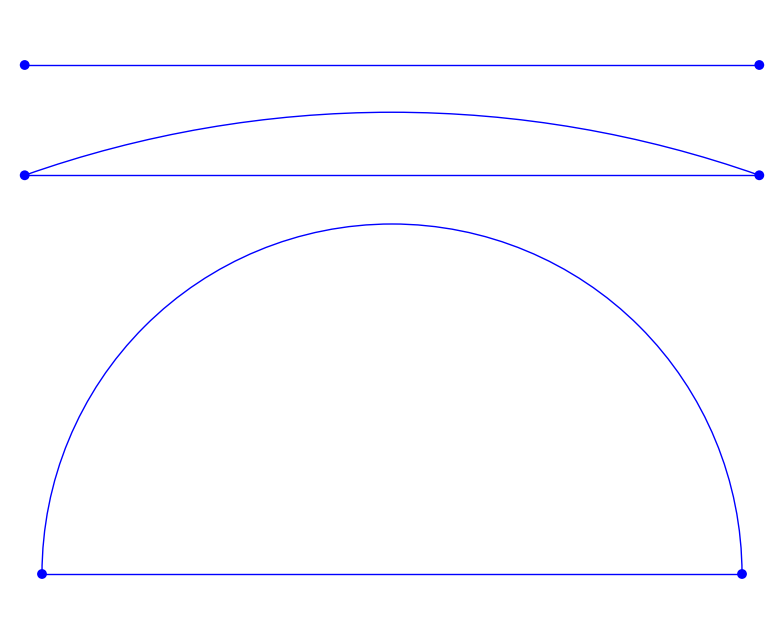
\includegraphics[width=0.3\textwidth]{img/chord_arc.png}
\caption{\label{fg:chord_arc}From top to bottom, a straight line has equal distance and arc-length, small curvature implies slightly larger arc-length, and large curvature has much larger arc-length.}
\end{figure}

The (planar) Curve Shortening Flow is the evolution equation,
\[
\partial_t \gamma = - \kappa\nu
\]
for a smooth, one-parameter family of immersed curves $\gamma_t \subset \RR^2$ in the plane with $\kappa$ is the geodesic curvature with respect to a smooth choice of unit normal, $\nu$. The most famous result regarding this equation is that closed, embedded curves collapse to a point in finite time, smoothly converging to a circle after rescaling to keep the total length fixed \cite{MR840401,MR906392}. In \cite{MR2794630}, with Prof. Ben Andrews and using the chord-arc profile, Dr. Bryan proved a distance comparison principle leading to a curvature bound and subsequent direct proof of this result. A related flow is the flow,
\[
\partial_t \gamma = -\kappa\abs{\kappa}^{\alpha-1} \nu.
\]
This flow has greater non-linearity than the Curve Shortening Flow, and owing to the absolute value, has non-smooth speed for non-convex curves at points where the curvature vanishes. Convergence results for convex curves (where the speed is smooth) have been obtained \cite{MR1660843}, but the general case remains open and may be approached using the distance comparison methods of Prof. Ben Andrews and Dr. Bryan.

The distance comparison argument in \cite{MR2794630} applies also to the Curve Shortening Flow of networks, a topic that has received considerable attention in recent years \cite{MR2394409,MR2075985,MR2763716}. In this context, a network is an embedded graph in the plane. Each edge has vertices either lying on the boundary of a convex body (or on the circle at infinity), or meets precisely two other edges at a vertex and with equal angles of $2\pi/3$ (\emph{triple condition}). See figure \ref{fg:network}.
\begin{figure}[htb]
\centering
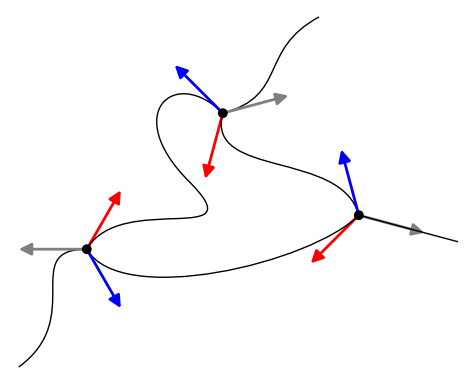
\includegraphics[width=0.4\textwidth]{img/network.png}
\caption{\label{fg:network}A network with three nodes satisfying the triple condition.}
\end{figure}

The flow is by curve shortening on the interior of the edges, subject to the boundary triple condition. Such a flow was initially studied to model annealing metals \cite{MR0078836} and is of interest in materials science. The flow, like in the smooth case, is also the gradient flow of the length functional, from which perspective the triple condition arises naturally. This part of the project aims to prove that singularity formation can only occur when an edge has length collapsing to zero, confirming the so-called multiplicity one conjecture.

This project's \textbf{aims} are:
\begin{enumerate}[label=\textbf{(A.\arabic*)}]
\item Investigate isoperimetric comparisons in negatively curved manifolds.
\item Define Homogeneous Curve Shortening Flow for non-convex curves and obtain convergence results by distance comparison.
\item Develop distance comparison for the Curve Shortening Flow of networks and investigate singularity formation.
\end{enumerate}

\noindent\textbf{Project B: Cross Curvature Flow (XCF) And Hyperbolic Manifolds}
\label{sec-2-2}
Let $E = \operatorname{Ric} - \tfrac{1}{2} \operatorname{R} g$ denote the Einstein tensor of a Riemannian manifold $(M, g)$. We define the endomorphism $\mathcal{E}$ of the tangent bundle $TM$ by $E(X, Y) = g(\mathcal{E}(X), Y)$, and Einstein-Ricci tensor,
\[
\operatorname{Ric}_E (X, Y) = \operatorname{Tr} \left[Z \mapsto \operatorname{Rm} (\mathcal{E}(Z), X) Y\right],
\]
Then the XCF is the evolution equation,
\[
\partial_t g = -2 \operatorname{Ric}_E.
\]
This is a parabolic equation and preserves negative sectional curvature \cite{MR2055396,MR2207496}. In three dimensions, negative sectional curvature corresponds to $E$ being a metric (positive definite bi-linear form), and the Einstein-Ricci tensor is nothing more than contracting the Riemann tensor, not with the metric $g$, but with the metric $E$. Note that contracting with $g$ gives the usual Ricci tensor and the flow becomes the celebrated Ricci flow. The XCF may in fact be defined in other equivalent ways that agree in three dimensions, but not in higher dimensions in a similar manner to the agreement of the Ricci flow and Yamabe flow in two dimensions. These higher dimensional flows have yet to be studied, opening the door for significant results in hyperbolic geometry of higher dimensions.

As noted in \cite{MR2602839}, hyperbolic manifolds are the largest class of prime manifolds, but it's not yet known whether this space is contractible, or even connected. The Cross Curvature Flow (XCF) was introduced in \cite{MR2055396} in the hopes of deforming negatively curved metrics $g_0$ on a compact three-manifold $M$ to constant curvature metrics. Such a conjectured result would confirm contractibility of the space of negatively curved metrics on a hyperbolic manifold. Partial results for homogeneous manifolds and solid tori have been established \cite{MR2407107,MR2653711,MR2602839} as well as asymptotic stability near hyperbolic metrics \cite{MR2448593} in support of the conjecture.

This project's \textbf{aims} are:
\begin{enumerate}[label=\textbf{(B.\arabic*)}]
\item Prove the XCF deforms classes of strictly negatively curved metrics to constant curvature metrics.
\item Determine isoperimetric comparisons for the XCF.
\item Generalise the XCF to higher dimensions.
\end{enumerate}

\noindent\textbf{Project C: Ancient Solutions}
\label{sec-2-3}
It has long been understood that curvature flows and minimal surfaces are closely related, yet explicit applications to minimal surfaces have been minimal. In \cite{2016arXiv160401694B}, Dr. Mohammad Ivaki, Dr. Julian Scheuer and Dr. Bryan proved the very general result that any convex, ancient hypersurface solution of a parabolic, geometric flow in the sphere must be a family of shrinking spherical caps emanating from an equator (a minimal surface) at $t=-\infty$ and collapsing to the north pole at $t=0$. To obtain similar results in a general Riemannian background, given an unstable minimal surface $M_0$, linear stability analysis implies that the space of ancient solutions converging backwards to $M_0$ as $t\to-\infty$ is a finite dimensional linear sub-manifold corresponding to the unstable eigenspace. Further analysis should show that there is unique mean convex ancient solution corresponding to the first eigenvalue which is simple (the eigenspace is one-dimensional).

This project's \textbf{aims} are:
\begin{enumerate}[label=\textbf{(C.\arabic*)}]
\item Classify ancient solutions of curvature flows in Riemannian backgrounds.
\item Prove area estimates for unstable minimal surfaces in terms of the space of unstable directions.
\item Develop applications of curvature flows to conformal spherical geometry.
\end{enumerate}

\smallskip\noindent{\Large\textbf{\textsc{Project Quality And Innovation}}}
\label{sec-3}

\noindent\textbf{Comparison theorems for the isoperimetric profile.}
\label{sec-3-1}
An innovation of this project is the use of Isoperimetric comparisons which may then be used to tackle problems such as the Aubin-Cartan-Hadamard conjecture mentioned above. One possible approach is to deform regions by curvature flows such as the Mean Curvature Flow or the Inverse Mean Curvature Flow. This approach was taken in \cite{MR2420018} by using the mean-convex Mean Curvature Flow to prove the Euclidean isoperimetric inequality but suffered from the lack of suitable tools to analyse non-smooth flows. Such tools have been developed recently for example in \cite{MR3570481,2013arXiv1304.0926H} where regularity results and structure theorems have been more fully developed.

A further exciting possibility is tied in with the Cross Curvature Flow project described in this proposal and better adapted to negative curvature than the Ricci flow. The aim is to develop a parabolic viscosity equation leading to comparisons similar to those developed for the Ricci flow and Curve Shortening Flow \cite{MR2729306,MR2843240,pbthesis,Bryan}. If the Cross Curvature Flow deforms the metric to constant curvature, then the isoperimetric profile also converges to the model case and suitable monotonicity would prove the Aubin-Cartan-Hadamard conjecture.

\noindent\textbf{Homogeneous Curve Shortening Flow}
\label{sec-3-2}
For the homogeneous Curve Shortening Flow, an innovation is to define approximating flows,
\[
\partial_t \gamma = -\kappa\abs{\kappa^2 + \epsilon^2}^{\tfrac{\alpha-1}{2}} \nu
\]
which are smooth, strictly parabolic flows. The next step is to obtain a priori estimates via two approaches: one for $\alpha \in (1/3, 1]$ and one for $\alpha \geq 1$. Both methods are applicable to the critical case of the Curve Shortening Flow, $\alpha = 1$, the first method being the distance comparison principle in \cite{MR2794630}.

For such flows, the comparison applies for \emph{operator monotone} functions which satisfy $A \geq 0 \Rightarrow f(A) \leq 0$ for matrix $A$, which restricts to $\alpha \leq 1$. The following differential inequality for the chord-arc profile holds in this case:
\[
\partial_t Z \geq 2 \frac{2^{\alpha+1}}{\left(\sqrt{1 - (Z')^2}\right)^{\alpha-1}} f(Z'') - \avg{f(\kappa) \kappa} \left(Z - Z'\ell\right) - Z' \int_{p_0}^{q_0} f(\kappa)\kappa ds
\]
where $f(y) = y\abs{y}^{\alpha-1}$ is the speed of the flow, $\avg{\cdot}$ denotes the mean value over the curve $\gamma$ and $(p_0, q_0)$ are points of given intrinsic length $\ell(p_0, q_0)$ achieving the infimum of extrinsic distance $d(p_0, q_0)$. Given the critical exponent $\alpha=1/3$ discussed above, it's expected that the curvature estimates obtained using the methods in \cite{MR2794630} should hold for $\alpha \in (1/3, 1]$. Supporting evidence for this conjecture is that the differential inequality is linearly stable around the round circle.

For the case $\alpha \geq 1$, the Harnack inequality may be used (similar to \cite{MR1094458}) to show that the approximating flows become convex in finite time whence the existing results for convex curves apply.

\noindent\textbf{Network Curve Shortening Flow}
\label{sec-3-3}
Preliminary work by Prof. Mariel \saez{} and Dr. Bryan have shown that a comparison principle for the chord-arc profile developed in \cite{MR2794630} holds for networks. Let us write $\Delta v_m$ for the tangential speed at vertices. Then the viscosity equation for the chord-arc profile is
\[
\partial_t Z \geq 4Z''+\bar{Q}(Z-xZ')+f'(\Delta Q(p,q)).
\]
where $\bar{Q}=\frac{1}{L}\int k^2 ds-\sum_{m=1}^n \Delta v_m$ and $\Delta Q(p,q)=\frac{1}{L}\int_p^q k^2 ds-\sum_{m=i_p}^{i_q} \Delta v_m$. The only difference with the smooth case is the introduction of the $\Delta v_m$ terms.

Two important differences however are that the asymptotics of the chord-arc profile differ from the smooth case and that the triple points introduce new terms into the viscosity equation. An important innovation here, only guess at in \cite{MR2794630}, is to apply a powerful procedure for finding suitable comparison functions: make a similarity substitution using the profile of the self-similar solution in the viscosity equation which handles has the advantage of automatically building in the two differences to the comparison.

\noindent\textbf{The Cross Curvature Flow and hyperbolic manifolds}
\label{sec-3-4}
The project on the Cross Curvature Flow and hyperbolic manifolds is highly innovative, identifying previously unknown deep structure and describing powerful techniques for understanding the geometry of hyperbolic manifolds similar to the Ricci flow's role in positively curve geometry. The extensions to higher dimensions and underlying algebraic structure have not previously been observed and will open up an entirely new approach to high dimensional hyperbolic geometry. Furthermore, the isoperimetric comparisons will demonstrate that the tremendous power of these methods has very broad applicability building upon my previous innovations.

\subsubsection*{Harnack Estimates}
\label{sec-3-4-1}
The conjectured asymptotic behavior of the XCF has been recently confirmed whenever $M$ locally isometrically embeds as a hypersurface into Minkowski space $\RR^{3,1}$ \cite{MR3344442}. The main observation there is that in such a situation, the embedded hypersurface evolves by the Gauss curvature flow. In this situation, Dr Mohammad Ivaki, Dr. Julian Scheuer and Dr. Bryan obtained the Harnack inequality \cite{BIS4},
\[
\partial_t \sqrt{{\det} \mathcal{E}} - \frac{1}{\sqrt{{\det}\mathcal{E}}} \abs{\nabla \sqrt{{\det}\mathcal{E}}}_E^2  + \frac{3}{4 t} \sqrt{{\det}\mathcal{E}} \geq 0
\]
where $\abs{\cdot}_E$ refers to the norm with respect to the Einstein tensor $E$. An immediate application of this inequality is that negative sectional curvature is preserved by the flow as if becomes $\mathcal{E}$ singular, the Harnack inequality implies $\nabla \mathcal{E}$ blows up. Moreover, combined with $C^0$ estimates, the Harnack inequality gives an alternate proof of the conjecture. Thus a general Harnack inequality is needed. Proving the Harnack involves great computational complexity in the general case, though early computations show it is possible to obtain a Harnack under the assumption, $\nabla V$ is totally symmetric where $V (X, Y) = g(\mathcal{E}^{-1}(X), Y)$ which is automatically satisfied n the locally embedible by the Codazzi equation. These initial results are already more general than those in \cite{MR3344442} and will be an early output of the project when developed more fully.

\subsubsection*{Comparisons for the Einstein volume under the Cross Curvature Flow.}
\label{sec-3-4-2}
An innovation, connected with the isoperimetric comparisons part of this proposal is to derive a viscosity equation for the Einstein Isoperimetric Profile:
\[
I_E (x) = \inf\{\operatorname{Area}_E (\Omega) : \operatorname{Vol}_E (E) = x\}
\]
where the area and volume are measured with respect to the Einstien tensor $E$. In \cite{MR2055396} it was shown that the Einstien volume is monotone along the flow, which suggests that as with the isoperimetric profile for the Ricci flow, this approach will prove quite powerful.

\subsubsection*{Higher Dimensions}
\label{sec-3-4-3}
The definition given above for the XCF makes sense in any dimension. Moreover, there is another way to interpret the XCF. First recall above that the XCF is the equation,
\[
\partial_t g = -2 \operatorname{Ric}_E.
\]
Let us call this equation the \emph{Einstein Ricci Flow}. Now, let $\operatorname{adj} \mathcal{E}$ denote the adjugate of $\mathcal{E}$ defined as the $\wedge$ adjoint of $\wedge^{n-1} \mathcal{E}$:
\[
\operatorname{adj} \mathcal{E} (X) \wedge \eta = X \wedge (\wedge^{n-1} \mathcal{E}) \eta
\]
for any tangent vector $X$ and $n-1$ vector $\eta$. Writing $\operatorname{adj} E (X, Y) = g(\operatorname{adj} \mathcal{E} (X), Y)$, we define the \emph{adjugate Einstein flow}:
\[
\partial_t g = \operatorname{adj} E.
\]
In the critical dimension three, by diagonalising $\operatorname{Ric}$, one finds that $\operatorname{adj} E = -2\operatorname{Ric}_E$ so that both flows agree. In higher dimensions however this is no longer true. This should be compared with the Ricci flow and Yamabe flow which agree in the critical dimension, two but differ in higher dimensions. The aim here is to develop a theory of the XCF in higher dimensions strictly negative curvature operator and/or vanishing Weyl tensor are related to the positive definiteness of $E$ giving natural conditions to impose in the initial study.

\noindent\textbf{Ancient Solutions and Minimal Surfaces}
\label{sec-3-5}
An important innovation in this part of the proposal is to use linear stability analysis of the Mean Curvature Flow near an unstable minimal surface to produce ancient solutions. Such techniques were first used to prove forward convergence results \cite{MR1485470} and the novelty here is to show that corresponding to the negative eigenspace is a linear, invariant manifold containing all ancient solutions emanating from an unstable, closed minimal surface. What's more, corresponding to the first eigenvalue - whose eigenspace is one-dimensional - there exists a unique mean-convex ancient solution of the mean curvature flow.

Conversely, assuming bounds on the second fundamental form $\abs{A} \leq M$ for an ancient solution, compactness results should produce a limiting hypersurface $M_0$ at $t=-\infty$. In the particular case of mean convex ancient solutions, the flow is monotone and hence $M_0$ is unique and a partial classification may be so obtained. When a suitable Harnack inequality holds for a convex ancient solution, the assumed bound on $\abs{A}$ follows directly.

A completely new idea introduced here is now to use such classification results, particularly in the mean convex case to obtain estimates for minimal surfaces. Geometric inequalities for a minimal surface $M_0$ bounding a region $\Omega_0$ may be obtained similarly to \cite{MR1650335} by integrals of the form
\[
\text{Vol}(\Omega_0) \leq \int_{\text{Area}(M_T)}^{\text{Area}(M_0)} f(x) dx
\]
where the integrand $f$ is deduced from model comparisons obtained by estimates of the Willmore energy $\mathcal{W} = \int H^2$ which arises naturally from the variation of area under the Mean Curvature Flow,
\[
\partial_t \text{Area} = -\int H^2.
\]
Here $T$ denotes the first singular time, but using new results for mean convex mean curvature flow \cite{2013arXiv1304.0926H,MR3570481}, one may extend the integral past $T$ to the time when the mean convex solution becomes extinct, at which point $\text{Area}(M_T) = 0$. Thus one obtains estimates depending only on the $\text{Vol}(M_0)$ and $\text{Area}(M_0)$.

As a striking example of possible further innovative applications, the methods described produce a five-dimensional family of ancient solutions emanating from a Clifford Torus in $\sphere^3$. The motion of this family is, to first order, by the canonical family of conformal transformations used in the resolution of the Willmore conjecture \cite{MR3152944}. This suggests a hitherto unknown connection between the conformal geometry of the sphere and the Mean Curvature flow with applications to Willmore surfaces.

\smallskip\noindent{\Large\textbf{\textsc{Decra Candidate}}}
\label{sec-4}
The MSI will host the candidate during this grant and will make up the shortfall in salary between the DECRA salary and the position at MSI. The teaching and administrative requirements are minimal, allowing the candidate more time to focus on research than has been available to him in the past. At this stage, the candidate will hold no other grants and will have no additional responsibilities besides the teaching and administrative requirements already mentioned. This will allow the candidate to focus his energies on conducting research, allowing him ample time to establish and implement the research program.

\smallskip\noindent{\Large\textbf{\textsc{Feasibility}}}
\label{sec-5}
The project builds on the candidate's existing expertise in isoperimetric problems and curvature flows \cite{Bryan,pbthesis,MR2843240,MR2794630,MR2729306} as well as Harnack inequalities and ancient solutions \cite{BIS4,bryanlouie,2016arXiv160401694B,2015arXiv150802821B,2015arXiv151203374B}. The methods were developed by the candidate and collaborators and have a high chance of producing strong research outcomes, building on proven techniques published in top journals. The aims are ambitious, but involve many intermediate steps along the away, some of which already have been established, ensuring continual progress throughout the duration of the project. The aims closely align with the expertise of the MSI, particularly Prof. Ben Andrew with whom the candidate has already established a strong and successful research program.

\smallskip\noindent{\Large\textbf{\textsc{Benefit}}}
\label{sec-6}
The funding requested is minimal, consisting principally of salary and a modest request for travel. Hence the execution of the of the project offers excellent value for money, particularly as the candidate's research to date shows the methods described in this proposal are extremely effective. 

The research is highly innovative, with strong results already obtained by these methods, and involves international collaboration strengthening Australia's ties with research institutes in North and South America, Europe and China. The techniques developed also have very broad applicability, as has already been established by the candidate's previous work, and hence benefits the international community in pushing the frontiers of geometric and non-linear analysis. Australia in particular will see social, cultural and economic benefits by strengthening it's international reputation and attracting leading researchers and students to Australia to study the innovative new methods developed in the project.

\smallskip\noindent{\Large\textbf{\textsc{Communication Of Results}}}
\label{sec-7}
The results of the project will be disseminated primarily by scholarly publications in high quality journals similar to level of the candidates existing publications. Direction communication with the international research community will take place via conferences, workshops and seminars.

\smallskip\noindent{\Large\textbf{\textsc{Management Of Data}}}
\label{sec-8}
The outcomes of this project will be posted to the arXiv pre-print server (\url{http://arxiv.org/}) where they will be freely available to the general public and published in top quality refereed mathematical journals.

\printbibliography
% Emacs 24.5.1 (Org mode 8.2.10)
\end{document}
